\section{Big Code}
\paragraph{Big Code:} Create new software tools that leverage massive codebases to solve
problems beyond what is possible with traditional techniques. Usually the more specifications (understanding of how program code works) to standard models the better they get. The goal is to learn specifications automatically from large codebases.
\subsection{Example: Injection Attacks}
\paragraph{Tools to find Injection Attacks}
Use static taint analysis, but what about missing (not detected) sinks, sanitizers and sources? \\

\begin{minipage}{0.9\linewidth}
    \centering      
    \def\svgwidth{\columnwidth}
    %% Creator: Inkscape 1.0 (4035a4fb49, 2020-05-01), www.inkscape.org
%% PDF/EPS/PS + LaTeX output extension by Johan Engelen, 2010
%% Accompanies image file 'L10_Model.pdf' (pdf, eps, ps)
%%
%% To include the image in your LaTeX document, write
%%   \input{<filename>.pdf_tex}
%%  instead of
%%   \includegraphics{<filename>.pdf}
%% To scale the image, write
%%   \def\svgwidth{<desired width>}
%%   \input{<filename>.pdf_tex}
%%  instead of
%%   \includegraphics[width=<desired width>]{<filename>.pdf}
%%
%% Images with a different path to the parent latex file can
%% be accessed with the `import' package (which may need to be
%% installed) using
%%   \usepackage{import}
%% in the preamble, and then including the image with
%%   \import{<path to file>}{<filename>.pdf_tex}
%% Alternatively, one can specify
%%   \graphicspath{{<path to file>/}}
%% 
%% For more information, please see info/svg-inkscape on CTAN:
%%   http://tug.ctan.org/tex-archive/info/svg-inkscape
%%
\begingroup%
  \makeatletter%
  \providecommand\color[2][]{%
    \errmessage{(Inkscape) Color is used for the text in Inkscape, but the package 'color.sty' is not loaded}%
    \renewcommand\color[2][]{}%
  }%
  \providecommand\transparent[1]{%
    \errmessage{(Inkscape) Transparency is used (non-zero) for the text in Inkscape, but the package 'transparent.sty' is not loaded}%
    \renewcommand\transparent[1]{}%
  }%
  \providecommand\rotatebox[2]{#2}%
  \newcommand*\fsize{\dimexpr\f@size pt\relax}%
  \newcommand*\lineheight[1]{\fontsize{\fsize}{#1\fsize}\selectfont}%
  \ifx\svgwidth\undefined%
    \setlength{\unitlength}{720.00000454bp}%
    \ifx\svgscale\undefined%
      \relax%
    \else%
      \setlength{\unitlength}{\unitlength * \real{\svgscale}}%
    \fi%
  \else%
    \setlength{\unitlength}{\svgwidth}%
  \fi%
  \global\let\svgwidth\undefined%
  \global\let\svgscale\undefined%
  \makeatother%
  \begin{picture}(1,0.5625)%
    \lineheight{1}%
    \setlength\tabcolsep{0pt}%
    \put(0,0){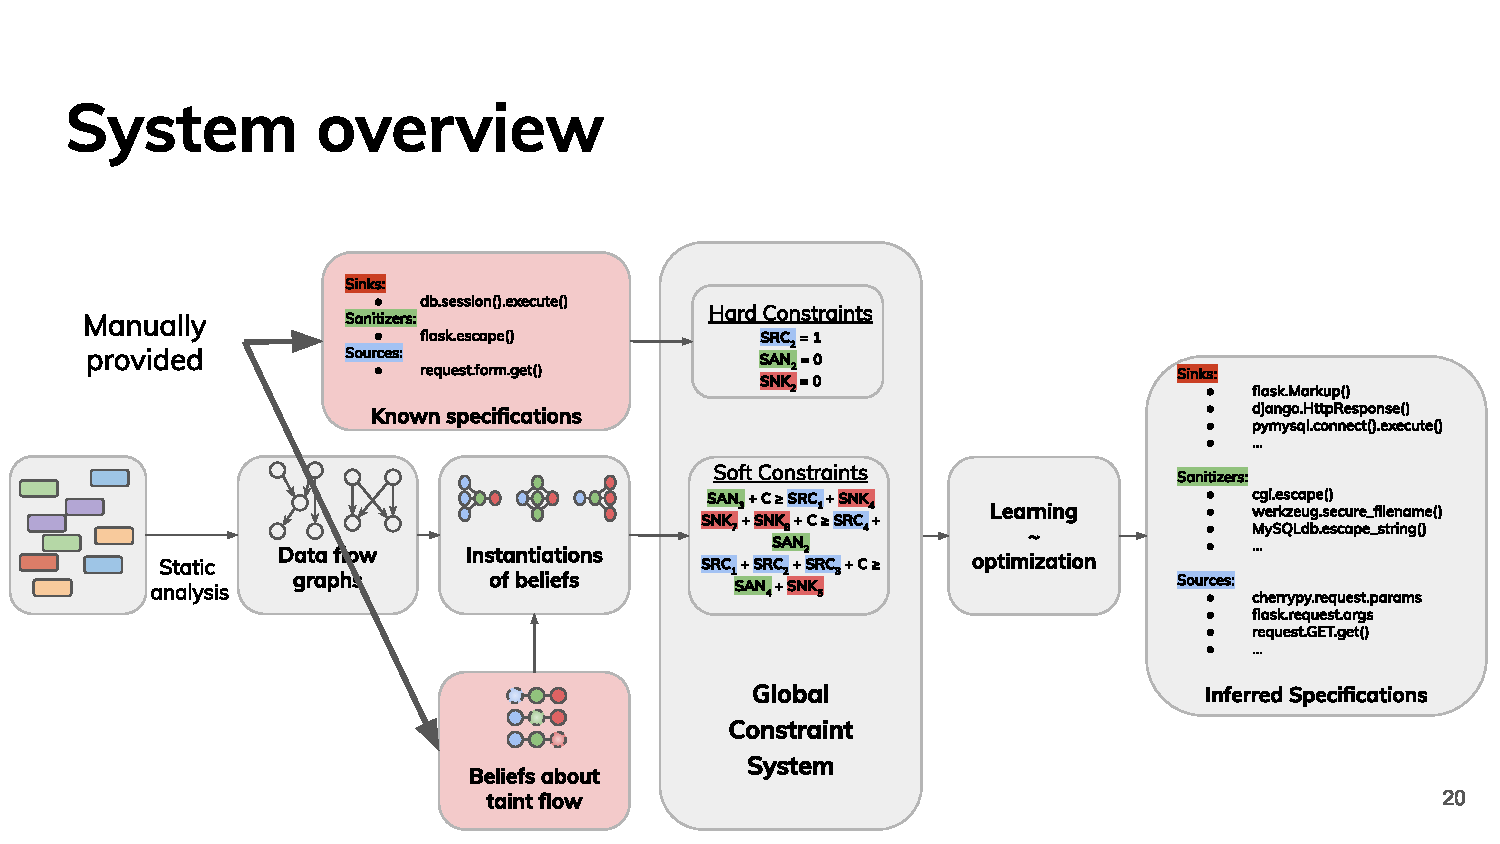
\includegraphics[width=\unitlength,page=1]{L10_Model.pdf}}%
  \end{picture}%
\endgroup%    
\end{minipage}

\subsection{Pointer Analysis}
\paragraph{Problems with Pointer Analysis:}
\begin{itemize}
    \item Analysis of code for different libraries.
    \item Dynamic Runs (e.g. complex runtime behaviours of java.sql)
    \item Need knowledge how to analyze corner cases and libraries
\end{itemize}
\\
$\rightarrow$ Use ML for a scalable solution to pointer analysis!
